\documentclass[]{article}
\usepackage{epsfig}
\usepackage{graphicx}
\usepackage{natbib}

\parskip 0.1in
\parindent 0.0in
\setcounter{secnumdepth}{1}
\title{Deep Learning}

\author{Yann LeCun, Yoshua Bengio, Geoffrey Hinton}

\begin{document}

\maketitle

\section{Preface}

Deep neural networks that learn many layers of feature detectors have
dramatically improved the state-of-the-art for speech recognition, object
recognition, object detection, predicting the activity of drug molecules,
and many other tasks. Deep learning discovers intricate structure in large
datasets by using the backpropagation algorithm to compute
error-derivatives for the weights that define each feature detector and
then repeatedly change these weights in proportion to their derivatives
averaged over small batches of training examples.  Deep recurrent neural
networks, in which each layer also receives input from its own state at the
previous time-step, can now generate good captions for images and are
competitive for machine translation.

\section{Introduction}

Deep learning is currently making major advances in solving problems that
have resisted the best attempts of the Artificial Intelligence community
for many years. Deep learning is very good at discovering intricate
structure in large, high-dimensional datasets and is therefore widely
applicable in all of the sciences. For example, it has beaten previous
machine learning techniques at predicting the activity of potential drug
molecules~\cite{Dahl}, detecting new fundamental particles~\cite{??},
classifying galaxies~\cite{??}, or predicting the effects of mutations in
non-coding DNA on gene expression and disease~\cite{Frey}.

So far, most applications of deep learning use feed-forward neural
networks, but for tasks that involve sequential inputs it is often better
to use recurrent neural networks. These are given one element from an input % YB term-->element
sequence at each time step and their recurrent internal ``hidden'' state
depends on the whole history of the input sequence. Recurrent networks are
very good at predicting the next character in a string\cite{Sutskever} or
the next word in a sequence\cite{Mikolov} but they can also be used for
more complex tasks.  After reading an English sentence one word at a time,
for example, an English``encoder'' network can be trained so that the final
state vector of its hidden neurons is a good representation of the thought
expressed by the sentence.  This thought vector can then be used as the
initial hidden state of a trained French ``decoder'' network which outputs
a probability distribution for the first word of the French translation. If
a particular first word is chosen (e.g., according to that probability)
and provided as input to the decoder
network it will then output a probability distribution for the second word
of the translation and so on until a full stop is chosen~\cite{Vinyals,
  Montreal}. 
%YB added a clarification
Overall, this process generates sequences of French words according to
a probability distribution that depends on the English sentence.

This rather naive way of performing machine translation has quickly become
competitive with the state-of-the-art and this raises serious doubts about
whether understanding a sentence requires anything like internal symbolic
expressions that are manipulated by binding their symbols to the variables
in judiciously chosen rules of inference.  The encoder-decoder translation
networks do not work by using internal rules of inference in which
variables get bound to symbols. They just use big state vectors, big weight
matrices and scalar non-linearities to get the job done.  This suggests
that deriving conclusions using only the form of the premises is a powerful
technique that people can eventually master but it is not a good model of
the way we normally reason or understand language. Recurrent neural
networks that represent thoughts as big vectors are more compatible with
the view that everyday reasoning involves many simultaneous analogies that
each contribute plausibility to a conclusion\cite{metaphors}.

This review is organized chronlogically starting with the introduction of
the backpropagation algorithm in the 1980's. After describing some of its
early successes, we explain the actual and perceived limitations that
prevented it from living up to its early promise for so many years and how
these limitations were eventually overcome.

\section{Pattern recognition and the back-propagation algorithm}

Patterns can be classified by first converting each raw input vector into a
vector of feature activations and then collecting evidence for each
possible class by computing a weighted sum of the features. If good
features can be designed by hand, it is relatively easy to learn
class-specific weights that optimize
discrimination~\cite{perceptrons}. Widely-used examples of such linear
classification methods are logistic regression and linear support vector
machines~\cite{logisticregression,svm}.

However, even with good hand-crafted features, many interesting tasks
cannot be solved by linear classifiers. A common method to get around this
problem is to transform the feature vector into a higher dimensional vector
through a non-linear mapping, exploiting the fact that collections of
vectors are more likely to be easily spearated when they are spread around
a high-dimensional space~\cite{cover}. One clever way to do so is to use a
``kernel function'' that measures the similarity between two vectors.
Using the kernel function, any input vector, ${\bf x}_i$ in the training
set can be used to define a feature whose activation for a new input
vector, ${\bf x}_{\rm new}$ is just the similarity between ${\bf x}_i$ and
${\bf x}_{\rm new}$. Given a kernel function, it is possible to jointly
optimize the choice of training inputs used to define features and the
class-specific weights associated with the features~\cite{svm}. The training
inputs used to define features are called ``support vectors'' and Support
Vector Machines\cite{Vapnik} have been very successful, especially for
tasks with a relatively small number of training examples in which features
are individually informative. They do not, however, perform well for tasks
such as object recognition in which the input space is high-dimensional and
the input-output mapping is so complex that computing similarities with a
simple kernel function is ineffective.

Problems such as image and speech recognition require the input-output
function to be insensitive to irrelevant variations of the input, such as
variations in position, orientation or illumination of an object, or
variation in pitch or accent of speech, while being very sensitive to
particular minute variations, such as the difference between a white wolf
and a samoyed dog. These tasks are better handled with multiple layers of
progressively more complicated feature detectors each of which is defined
in terms of the simpler feature detectors in the previous layers.

From the earliest days of pattern recognition~\cite{selfridge,Rosenblatt57}
researchers aimed to replace hand-engineered features by multiple layers of
learned features.  This was eventually achieved by using the
backpropagation algorithm which was discovered independently by several
different groups in the 1970s and 1980s\cite{Werbos74,Parker85,LeCun85,Rumelhart86b,schmidreference}.  Backpropagation is simply an application of
the chain rule, which yields an efficient way of computing the gradient of a
smooth objective function with respect to all of the weights in a layered
network. The objective function typically measures the discrepancy between
the actual output of the network on a given training case and the target
output for that case.  The key insight is that the error derivatives with
respect to the {\it outputs} of a layer can be computed by working
backwards from the error derivatives with respect to the outputs of the
subsequent layer. Once this backwards recursion has been used to compute
error derivatives for the outputs of all layers, it is easy to compute
error derivatives for the parameters (or weights) of each layer (see box
1).

%%%%%%% GEOFF %%%%%%%%%%
GEOFF: Do box explaining backprop equatons
%%%%%%%%%%%%%%%%%%%%%%

\section{Stochastic gradient descent}

Backpropagation provides an efficient way of computing gradients for all of
the weights in a layered network on a single training case, but there are
still many ways to make use of these gradients. The most obvious method is
to average the gradients over all of the cases in the training set and then
to change each weight in proportion to its negative gradient, which is the
direction where a small change will most improve the objective function. 
When the training set contains millions of cases and is highly redundant, however,
this is needlessly slow. It is much faster to compute the average gradient
on a small ``mini-batch'' of randomly chosen training cases and to update
each weight by this stochastic estimate of its full gradient times a
learning rate which decays as learning proceeds. Stochastic gradient
descent can be improved by using the history of the individual weight
gradients to adapt the learning rate for each weight~\citep{bottou-bousquet-2008-small}
or to provide additional increments that depend on earlier gradients\cite{momentum}
but these techniques are still the subject of controversy and are beyond
the scope of this review.  However, it is now widely accepted that some
form of stochastic gradient descent is the best bet for large, redundant
datasets.

\section{Distributed representations}

The hidden layers of a multi-layer neural network learn to represent the
network's inputs in a way that makes it easy to predict the target
outputs. This is nicely demonstrated by training a multi-layer neural
network to predict the next word in a sequence from a local context of
earlier words~\citep{BenDucVin01-short}. 
Each context word is presented to the network as a one-of-N
vector in which one component has a value of $1$ and the rest are $0$. The
output layer has one unit per word and is forced to produce a probability
distribution over words by using the ``softmax'' function:
\begin{equation}
p_j = \frac{exp(z_j)}{\sum_i exp(z_i)}
\end{equation}
where $z_j$ is the total input received by output unit $j$. The hidden
layers use either the logistic or tanh non-linearity:
\begin{equation}
y_j = \frac{1}{1+ \exp(z_j)}, \ \ \ y_j = \frac{}{} % YB: what was the intent here for the 2nd part?
\end{equation}

The connectivity of the network is restricted so that each of the one-of-N
input vectors must first be converted to a ``word-vector'' before being
used by subsequent layers to give a high probability to the target next
word.  The network learns word-vectors that contain many active components
each of which can be interpreted as a separate feature of the word. This
was first demonstrated\cite{RHW} using sequences of three words, such as
(Colin, Mother, Victoria), derived from two family trees. The learned word
vector for Colin contained ``semantic'' features representing which family
tree Colin was in, what branch of that tree he was in, and from what generation
he was~\cite{Hinton-et-al-PDP1986}. These semantic features were not explicitly present
in the input.  They were discovered by the learning procedure as a good way
of factorizing the structured relationships between the input and output
symbols into multiple ``micro-rules''.  For example, given Colin's
generation and the learned feature of Mother that the output should be one
generation higher than the input, we can already restrict the answer to
people in a specific generation. The ability of deep learning to discover
many such micro-rules allows it to generalize well to novel combinations of
individually familiar context words.

The family tree demonstration used a small, clean dataset in which the
regularities could be captured by micro-rules that were never violated and
the features were easy to interpret, but learned word-vectors also work
very well when the word sequences come from a large corpus of real text and
the individual micro-rules are unreliable~\citep{BenDucVin01-short}. When trained to
predict the next word in a news story, for example, the learned word
vectors for Monday and Tuesday are very similar, as are the word vectors
for Vietnam and Iraq.  Vector representations of words learned from text
are now very widely used in natural language applications~\cite{Schwenk-2007,CollobertR2008-short,
Mikolov-Interspeech-2011-small,Socher-2011}.

The issue of representation lies at the heart of the debate between the
logic-inspired and the neurally-inspired paradigms for cognition. In the
logic-inspired paradigm, an instance of a symbol is something whose only
property is that it is either identical or non-identical to other symbol
instances. It has no internal structure that is relevant to its use. By
contrast, neural networks use large activity vectors instead of symbols and
parallel matrix operations followed by non-linearities instead of formal
rules of inference. The elements of such vectors can be understood as
the values of learned attributes (or features) associated with some object. 
With sufficient data, computational power and depth,
the combination of backpropagation for computing gradients and stochastic
gradient descent for updating the weights on connections has proved to be
very good at learning appropriate distributed representations. These
representations allow a lot of parallel computation at the feature level so
that complex tasks can be solved in a very small number of sequential
steps. In fact, it can be shown that a measure of the richness of the functions
that can be represented by a deep neural network grows exponentially
with depth~\citep{Montufar-et-al-NIPS2014}.

\section{Convolutional neural networks}

%%%%%%%% YANN %%%%%%% 

YANN: can you summarize convnets and their use for reading cheques in about
350 words?

\citep{LeCun89-small}

%%%%%%%%%%%%%%%%%%%% 

\section{Recurrent Neural Networks}

When backpropagation was first introduced, its most exciting use was for
training recurrent neural networks. These receive input vectors at each
time-step and have one or more layers of hidden units that, in addition to
having connections to higher layers or ouput units, also have connections
that allow the neurons within a layer to receive weighted input from those
same neurons at the previous time-step.  The gradient for a recurrent
weight, $w_{ij}$ that allows neuron $i$ at time $t$ to influence the
activity of neuron $j$ at time $t+1$ can be computed by
backpropagation-through-time (BPTT) of the error derivative for $j$ at time
$t+1$. The full gradient for $w_{ij}$ on a whole input sequence is just the
sum of its gradients at each time-step.

Recurrent neural networks are very powerful dynamical systems, but training
them with BPTT proved to be problematic, because the backpropagated
gradients either grow or shrink at each time step, so over many time-steps
they typically explode or vanish~\cite{Bengio-trnn93-small,Hochreiter91-small}.

\section{Overcoming the limitations of backpropagation in deep networks}

In the 1990s, the machine learning community decided that backpropagation
in deep neural networks did not work well in practice and it was largely
abandoned.  At the time, people believed that learning many layers of
non-linear feature detectors with no prior knowledge was much too difficult
for a simple gradient descent procedure and that the networks were getting
trapped in poor local minima. We now know that the main reasons for the
limited success of backpropagation in deep networks were quite different:
The labeled datasets were far too small, the computers were far too slow,
and the weights were not initialised sensibly.

The obvious weakness of gradient descent is that it can get trapped in poor
local minima, but in high-dimensional weight-spaces this is much less
common than getting stuck close to saddle points where the error surface
curves upwards in most directions but downwards in a few. Recent
results~\cite{Dauphin-et-al-NIPS2014-small,Yann} strongly suggest
that in deep networks almost all of these local minima give very similar
performance so it does not matter which one we find.  This goes a long way
towards explaining why stochastic gradient descent works so well for deep
neural networks.

Interest in deep feed-forward networks was revived in 2005\cite{IJCAI} by
the introduction of an unsupervised learning procedure that could create
layers of feature detectors without requiring labeled data. The objective
in learning each layer of feature detectors was to be able to reconstruct
or model the activities of feature detectors (or raw inputs) in the layer
below.  By ``pre-training'' several layers of progressively more complex
feature detectors using this reconstruction objective, the weights of a
deep network could be initialized to sensible values.  A final layer of
output units could then be added to the top of the network and the whole
deep system could be fine-tuned using standard
backpropagation\cite{Science}. This worked remarkably well for recognizing
handwritten digits especially when the amount of labeled data was very
limited\cite{Bengio-nips-2006-small}.

The first major application of this pre-training approach was in speech
recognition and it was made possible by the advent of fast Graphics
Processing Units (GPUs) that were convenient to program~\citep{RainaICML09-small}.  
In 2009, the approach was used to map short temporal windows of coefficients extracted
from a soundwave to a set of probabilities for the various fragments of
speech that might be represented by the frame in the center of the window.
It achieved record-breaking results on a standard speech recognition
benchmark that used a small vocabulary\cite{TIMITpaper} and was quickly
developed to give record-breaking results on a large vocabulary
task~\cite{Dahl}.  By 2012, versions of the deep net from 2009 were being
developed by many of the major speech groups\cite{SPS} and were already
being deployed in Android phones.  For smaller datasets, unsupervised
pre-training leads to significantly better generalization~\citep{Erhan+al-2010-small}, 
but once deep
learning had been rehabilitated, it turned out that large labeled datasets
did not need the pre-training stage, provided the scales of the initial
random weights were carefully chosen to avoid very large or very small
initial gradients.

Interest in recurrent networks (which are deep in time) was revived by
``Long Short Term Memory'' networks (LSTMs) that use special hidden units
whose natural behaviour is to remember inputs for a long
time~\cite{Hochreiter+Schmidhuber-1997}.  
A linear ``memory cell'' interacts with other units
via gated connections whose weights are multiplied by the state of a
logistic gating unit that has an activation between $0$ and $1$. The input
vector has little effect on the state of a memory cell if the cell's input
gate has a low activation so memory cells can learn to selectively ignore
the input.  Similarly, a memory cell has little effect on the output if its
output gate has low activation. Each memory cell also has a connection to
itself (it is a leaky neuron) at the next time-step that has a weight of 1 so it tends to copy its
own real-valued state, but this self-connection is gated by a ``keep gate'' so
the stored value leaks quickly unless the keep-gate has an activation
near $1$.  The gates themselves have their activities determined by
weighted inputs that they receive from the input vectors and all of the
memory cells.

When LSTMs were first described in
English~\cite{Hochreiter+Schmidhuber-1997} their complexity was off-putting
and, despite their impressive ability to learn very long-range temporal
structure on toy problems, they were largely ignored until they achieved
excellent results in a competition to read cursive
hand-writing~\cite{Graves}. They have subsequently proved to be very
effective for tasks that have sequential input.  They are now better than
deep feed-forward networks for speech recognition~\cite{gravestimit} and
unlike feed-forward nets they can implement an entire speech recognition
system that goes all the way from coefficents derived from the soundwave to
the sequence of characters in the transcription~\cite{gravestimit}.  They
are also what is currently used for the encoder and decoder networks that
perform so well at machine
translation~\citep{Bahdanau-et-al-arxiv2014,Sutskever-et-al-NIPS2014}.

Recent work~\citep{Chung-et-al-NIPSDL2014} suggests that not all the elements of the LSTM
architecture are required, the crucial element being the presence of
of the gate controlling the leaking rate (or time constant) of the cell.
%It is not yet clear which aspects of the complicated architecture of LSTMs
%are really necessary. Memory cells are a good way of allowing the
%backpropagated error derivatives to neither explode nor vanish, but they
%are not the only way.  For example, recurrent nets with rectified linear
%hidden units that use the non-linear function $y=max(0,x)$ are much simpler
%than LSTMs and if the recurrent weight matrix is initialized to be close to
%the identity matrix they work about as well as LSTMs both for toy problems
%involving very long-range temporal structure and for real tasks like
%predicting the next word in text\cite{LeHinton}.


\section{Object recognition and detection with deep convolutional networks}

When deep convolutional networks were applied to a dataset of about a
million images from the web that contained a thousand different classes
they achieved spectacular results, almost halving the error rates of the
best computer vision sytems~\cite{kriz}.  Some of the images and the
network's predictions are shown in figure ??.  The major factors in this
success were the large labeled dataset~\cite{imagenet_cvpr09}, the use of fast GPUs,
and the convolutional early layers.  It had already been shown that deep
supervised nets with rectified linear units could be trained without
unsupervised pre-training~\citep{Glorot+al-AI-2011-small}. 
These rectified linear units made the
training much faster and the fully connected final layers were prevented
from overfitting the peculiarities of the training set by randomly omitting
hidden units during training~\cite{dropoutJMLR}. Deep convolutional nets
have quickly replaced the carefully engineered pipelines full of
hand-designed features developed by the computer vision community and they
are now deployed in many computer vision applications, including image
tagging, object detection, face recognition, facial expression recognition
and scene parsing.

%%%%%%%% YANN %%%%%%%
YANN: Add about 300 words plus another part of the figure showing detected
parts of people.
%%%%%%%%%%%%%%%%%%%%

\section{Language processing with deep networks}

\iffalse
%%%%%%%% YOSHUA %%%%%%%
YOSHUA: Add about 300 words plus t-sne figure of words and/or phrases.

The intro already explained the simple version of translation using encoder
and decoder nets and I suggest we save your ``translating with attention''
for introducing attention in the the future section.

After your stuff on language, I would like to include some version of the
paragraph below along with a figure.
%%%%%%%%%%%%%%%%%%%%%%%
\fi

Prior to the introduction of neural language
models~\citet{BenDucVin01-short} the standard approach to statistical
modeling of language was based on counting frequencies of occurences of
short symbol sequences (called n-grams). One disadvantage is that it
taking into account context beyond a handful of words would require
training corpora of exponentially growing size (with respect to the
desired context size), since the number of configurations of $n$
words from a vocabulary of size $V$ grows as $V^n$. Related to this
problem and the very notion of symbol introduced above, n-grams
do not generalize across the many semantically related sequences 
of words (for example the many ways of expressing roughly the same thing).
Instead, neural language models learn to associate each word to a
distributed representation (a vector) such that semantically related
words end up close to each other in that space, as illustrated in
Figure~\ref{fig:word-embeddings}. To obtain that effect, one
{\em jointly learns} a representation for each word as well as
a function that computes a quantity of interest that is relevant
to a language related task, such as predicting the next word
in a sequence (neural language models) or predicting the sequence
of translated words given the sequence of source words, i.e., neural
machine translation~\citep{Bahdanau-et-al-arxiv2014,Sutskever-et-al-NIPS2014}.


\begin{figure}[H]
\centerline{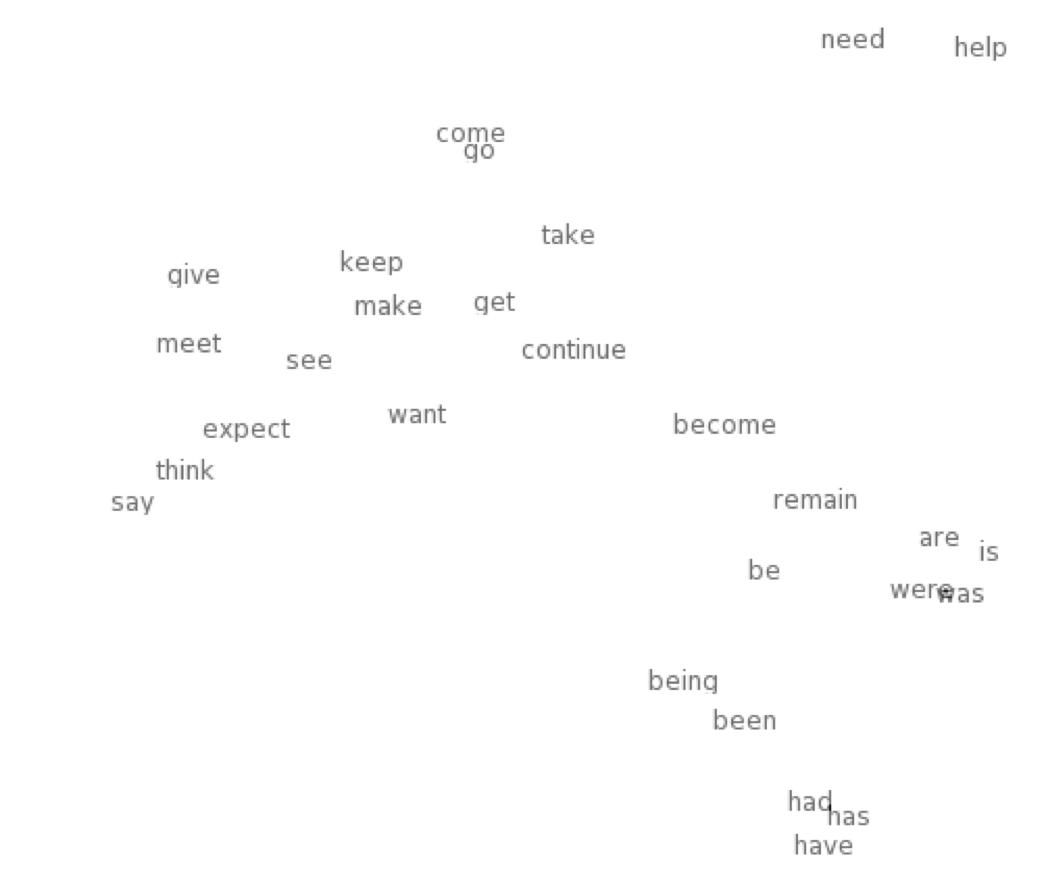
\includegraphics[width=0.7\linewidth]{word-embeddings.png}}
\caption{Illustration of word representations learned for modeling
language, non-linearly projected to 2-D for visualization using the
t-SNE algorithm~\citep{VanDerMaaten08}.}
\label{fig:word-embeddings}
\end{figure}

When translating between languages, the hidden units of the decoder network
that generates possible translations are initalized with a ``thought
vector'' which is the final hidden state of an encoder network.  But it is
also possible to initialize a decoder network using a linear transformation
of the last hidden layer of a deep convolutonal network that has already
been trained to recognize objects in images. The decoder network can then
be trained by BPTT on a dataset of captioned
images~\cite{NIC,StanfordNIC,more?} and it produces remarkably good
captions (see Figure~\ref{fig:caption-generation}).

\begin{figure}[ht]
%\centerline{\includegraphics[width=0.7\linewidth]{}}
\caption{Example of captions generated by a recurrent network taking
as extra input the representation extracted by a deep convolutional
net from an image, with the whole system trained to ``translate''
images into captions. Reproduced from~\citet{?}.
}
\label{fig:caption-generation}
\end{figure}


\section{Deep reinforcement learning}

Learning which action will maximize the total future reward given a state
of the world is difficult when the rewards are delayed and the world has a
very large number of possible states. One impressive recent development is
a single system that can learn to play many different video
games~\cite{NatureAtari}. The system uses a deep convolutional network to
map from the pixels on the screen at several previous time steps to the
expected future reward of each possible action and its only inputs are the
pixels and the current score in the game. The learning works by minimizing
the difference between the system's current estimate of future reward and a
noisy but less biased estimate that is obtained by using the same deep
network to estimate the future reward of the next state, where the next
state is chosen stochastically based on the predicted future rewards of all
the currently legal actions.

\section{Learning to process symbols}

Deep learning is now the method of choice for many perceptual tasks and is
making major inroads in natural language processing where a huge amount of
messy commonsense knowledge is required. Rapid progress is also being made
in applying deep learning, in particular BPTT, to relatively pure symbol processing tasks.
An impressive recent example is the ``Neural Turing Machine'' which is a
recurrent neural network that can choose when and what to write to or read
from an external memory~\cite{NTM}. Among other things, this can learn to
ouput a sorted list of symbols when its input consists of an unsorted
sequence in which each symbol is accompanied by a real value that indicates
its priority in the list.  To achieve this it must learn a sorting program
purely from examples of the input and output sequences.  A different system
that also uses BPTT can learn to map the sequence of characters in a simple
program written in Python to the sequence of characters that the program
would print~\cite{Woj}. Rather surprisingly, BPTT can learn about {\it for
  loops} and can also learn to perform addition and multiplication of
strings containing several decimal digits. Achieving this kind of behaviour
seemed ludicrously optimistic when BPTT was first proposed.
  
\section{The future of deep learning}

Human vision is an active process in which intelligent fixations are used
to ensure that only a tiny fraction of the optic array is ever processed at
high resolution. We expect much of the future progress in vision,
especially for video understanding or robotics, to come from systems that
are trained end-to-end and combine deep convolutional networks with
recurrent nets that use reinforcement learning to decide where to
look\cite{}.  Such systems already outperform passive vision
systems\cite{ba+mnih}.  Similarly, when understanding sentences or whole
documents we expect future systems to learn strategies for selectively
attending to one part at a time~\cite{Bahdanau-et-al-arxiv2014}. We also expect
that in the next few years deep recurrent neural networks will become far
better at understanding the meaning of documents, including the way in
which the thoughts expressed by the sentences are related to one another.

This review has focused on supervised learning because of its recent
achievements and we have ignored much interesting work on unsupervised
learning procedures for deep neural networks~\cite{deep-boltz, wake-sleep,
  google-cat, denoising-auto, ranzato-pami, more recent}. In the long run,
however, we believe unsupervised learning will be essential for allowing
deep networks to generalize well by creating internal representations that
untangle the many different factors that interact to produce images, speech
and documents~\cite{Yann,Bengio-Courville-Vincent-TPAMI2013}.

Finally, we believe that the recent successes of deep learning using
stochastic gradient descent are only the beginning.  As pointed out
in~\citet{Bengio+Lecun-chapter2007-small}, end-to-end learning
systems that have many parameters and few built-in assumptions can make use
of more data and more compute power far more easily than systems that
require hand-engineering of domain-specific knowledge.

 
%\section{Key references}
%{\it Quite a few of these are very recent and have not yet been published
%  through a peer-review so we are giving their arxiv references}.

%\subsection{Back-propagation and Stochastic Gradient Descent}

%Rumelhart, D. E., Hinton, G. E., \& Williams, R. J. (1986)\\ Learning
%representations by back-propagating errors.\\ {\it Nature}, {\bf 323},
%533-536.
% --> \citep{Rumelhart86b}

%LeCun, Y., Boser, B., Denker, J. S., Henderson, D., Howard, R.E., Hubbard,
%W., \& Jackel, L.D.\\ Backpropagation Applied to Handwritten Zip Code
%Recognition\\ Neural Computation, 1(4):541-551, Winter 1989
%--> \citep{LeCun89-small}

%\subsection{Distributed representations}

%Hinton, G. E., McClelland, J. L., \& Rumelhart, D. E. (1986)\\ Distributed
%representations.\\ In Rumelhart, D. E. and McClelland, J. L., editors, {\it
%  Parallel Distributed Processing: Explorations in the Microstructure of
%  Cognition. Volume 1: Foundations}, MIT Press, Cambridge, MA. pp 77-109.
% --> \citep{Hinton-et-al-PDP1986}

Bengio, Y., Ducharme, R., \& Vincent, P. (2001)\\ A neural probabilistic
language model.\\ In {\it NIPS 2000}, pages 932--938.

%% Collobert, R., Weston, J., Bottou, L., Karlen, M., Kavukcuoglu, K., Kuksa, P. (2011)\\
%% Natural language processing (almost) from scratch.\\
%% {\it The Journal of Machine Learning Research} 12, pages 2493-2537

Mikolov, T., Sutskever, I., Chen, K., Corrado, G.S., \& Dean
J.\\ Distributed representations of words and phrases and their
compositionality.\\ In {\it NIPS 2013}, pages 3111-3119.

Montufar, G.~F., Pascanu, R., Cho, K., and Bengio, Y. (2014).  On the
number of linear regions of deep neural networks.\\ In {\it NIPS'2014}.

\subsection{The apparent limitations of backpropagation in deep networks}

Bengio, Y., Simard, P., \& Frasconi, P. (1994)\\ Learning long-term
dependencies with gradient descent is difficult.\\ {\it IEEE Transactions
  on Neural Networks}, 5(2), 157-166.

%% Dauphin, Y., Pascanu, R., Gulcehre, C., Cho, K., Ganguli, S., and Bengio,
%% Y.\\ 
%% Identifying and attacking the saddle point problem in high-dimensional
%% non-convex optimization.\\ In {\it NIPS'2014}.

\subsection{Deep unsupervised learning}
Hinton, G., Osindero, S., \& Teh, Y. W. (2006)\\ A fast learning algorithm
for deep belief nets.\\ {\it Neural Computation}, 18(7), 1527-1554.

Erhan, D., Bengio, Y., Courville, A., Manzagol, P. A., Vincent, P., \&
Bengio, S. (2010)\\ Why does unsupervised pre-training help deep
learning?\\ {\it The Journal of Machine Learning Research}, {\bf 11},
625-660.

%% Mesnil, G., Dauphin, Y., Glorot, X., Rifai, S., Bengio, Y., Goodfellow, I.,
%% Lavoie, E., Muller, X., Desjardins, G., Warde-Farley, D., Vincent, P.,
%% Courville, A., and Bergstra, J. (2011).\\ Unsupervised and transfer learning
%% challenge: a deep learning approach.\\ In {\em JMLR W\&CP: Proc. Unsupervised
%%  and Transfer Learning\/}, volume~7.

\subsection{Deep speech recognition}

%% Mohamed, A. R., Dahl, G. E., \& Hinton, G. (2012)\\ Acoustic modeling using deep
%% belief networks.\\ {\it IEEE Transactions on Audio, Speech, and Language
%%  Processing}, 20(1), 14-22.

Hinton, G., Deng, L., Yu, D., Dahl, G. E., Mohamed, A. R., Jaitly, N. \&
Kingsbury, B. (2012)\\ Deep neural networks for acoustic modeling in speech
recognition: The shared views of four research groups.\\ {\it Signal
  Processing Magazine}, IEEE, 29(6), 82-97.


\subsection{Deep convolutional networks for image understanding}
LeCun, Y., Bottou, L., Bengio, Y., \& Haffner, P. (1998)\\ Gradient-based
learning applied to document recognition.\\ {\it Proceedings of the IEEE},
86(11), 2278-2324.

%% Jain, V., Seung, H.S., \& Turaga S.C. (2010)\\
%% Machines that learn to segment images: a crucial technology for connectomics\\
%% {\it Current opinion in neurobiology} 20 (5), 653-666.

Krizhevsky, A., Sutskever, I., \& Hinton, G. E. (2012)\\ Imagenet
classification with deep convolutional neural networks.\\ In Advances in
Neural Information Processing Systems (1097-1105).

%% Farabet, C., Couprie, C., Najman, L. \& LeCun, Y. (2013)\\
%% Learning Hierarchical Features for Scene Labeling,\\
%% IEEE Transactions on Pattern Analysis and Machine Intelligence, August 2013.

%% Sermanet, P., Eigen, D., Zhang, X., Mathieu, M., Fergus, R., \& LeCun,
%% Y. (2013)\\ Overfeat: Integrated recognition, localization and detection using
%% convolutional networks.\\ {\it Proceedings of ICLR 2014}, arXiv:1312.6229.

Tompson, J., Goroshin, R., Jain, A., LeCun, Y., \& Bregler, C. (2014)
Efficient Object Localization Using Convolutional
Networks. arXiv:1411.4280.


\subsection{Deep recurrent neural networks for text understanding and machine translation}

Graves, A., Liwicki, M., Fernández, S., Bertolami, R., Bunke, H., \&
Schmidhuber, J. (2009)\\ A novel connectionist system for unconstrained
handwriting recognition.\\ {\it IEEE Transactions on Pattern Analysis and
  Machine Intelligence}, 31(5), 855-868.

%% Devlin, J., Zbib, R., Huang, Z., Lamar, T., Schwartz, R., \& Makhoul,
% J. (2014)\\ Fast and robust neural network joint models for statistical machine
%% translation.\\ In {\it 52nd Annual Meeting of the Association for Computational
%%   Linguistics}, Baltimore, MD, USA.

Sutskever, I., Vinyals, O., \& Le, Q. V. (2014)\\ Sequence to sequence
learning with neural networks.\\ {\it arXiv preprint}, arXiv:1409.3215.

Bahdanau, D., Cho, K., \& Bengio, Y. (2014)\\ Neural machine translation by
jointly learning to align and translate.  {\it arXiv preprint},
arXiv:1409.0473.

Vinyals, O., Toshev, A., Bengio, S., \& Erhan, D. (2014)\\ Show and Tell: A
Neural Image Caption Generator.\\ {\it arXiv preprint}, arXiv:1411.4555.

%% Weston, J., Chopra, S., Bordes, A. (2014)\\
%% Memory Networks. arXiv:1410.3916.



\subsection{Deep reinforcement learning}
Mnih, V., Kavukcuoglu, K., Silver, D., Graves, A., Antonoglou, I.,
Wierstra, D., \& Riedmiller, M. (2013)\\ Playing Atari with deep
reinforcement learning.\\ {\it arXiv preprint} arXiv:1312.5602.

\newpage

\section{Boxes}

A box for the forward propagation and backpropagation equations.

\section{Figures}

1. Diagram showing:\\ a) A feedforward neural net.\\ b) A recurrent neural
net expanded in time.\\ c) A convolutional neural net.

2. Maps showing:\\ a) that word vectors learned by backpropagation are very
good at capturing the meanings of the words.\\ b) that the thought vectors
extracted by a translation model are very good at capturing the thoughts
expressed by sentences.

3. A diagram showing how unsupervised learning can be used to pre-train a
deep feeedforward neural net.

4. Some images with:\\ a) The opinions of a deep convolutional net about
the classes of the prominent objects.\\ b) Several alternative captions
generated by using the output of the convolutional net to determine the
initial hidden state of a decoder recurrent net.
 
5. Some images showing the localizations of parts of a person found by a
deep convolutional neural net.\\


\bibliography{strings,ml,aigaion}
\bibliographystyle{natbib}

\end{document}


